\documentclass[12pt,a4paper]{article}

\usepackage{buaa_paper}
\usepackage{fix-cm}


\schoolname{北京航空航天大学计算机学院}
\title{硕士学位论文文献综述}
\papertitle{基于神经网络的语言模型的性能优化研究}
\specialty{计算机科学与技术}
\studentnumber{SY1506330}
\researcharea{自然语言处理}
\advisor{荣文戈~~副教授}
\author{姜~~楠}
\date{2016 年 12 月 20 号}

\begin{document}

\maketitle



\addcontentsline{toc}{section}{摘要}
\keywords{神经语言模型;循环神经网络;层次多元概率模型}
{Neural Language Model;\ Recurrent Neural Network;\ Hierarchical Softmax}

\begin{abstract_ch}
语言模型是机器翻译和语音识别的主要应用领域。随着循环神经网络的发明,将其应用到语言模型上会使得语言建模更加精确,但是因此而带来的是模型速度下降。随着文本数据增大,单词的词表会变得十分巨大,导致计算代价非常大。历史上人们采用双层分类函数和多层分类函数来解决该问题,但是因此而带来的单词聚类问题变得更加苛刻。

本文首先介绍了语言模型的主要历史发展,回顾了自然语言处理领域中对上下文的建模、大词表问题的现有方案,以及历史上所采用的聚类模型主要模拟方法和算法。在建模方法中着重介绍了基于神经网络建模方法,即基于循环神经网络的建模方法。然后重点讨论了多层聚类算法的相关研究成果。最后本文还展望了对于不同算法的结合的成果和拟未来发展的几个方向。
\end{abstract_ch}
\newpage
\begin{abstract_en}
Historically, Language models has huge impact on machine translation or speech recognition. with the development of recent recurrent neural network, many researchers apply these advances on language model. Thus, there comes recurrent language models while they are lack of efficiency.  To be specific, when meeting with larger language model dataset, the vocabulary size becomes overwhelming time-consuming.

Traditionally, researchers utilise class-based softmax and tree-based hierarchical softmax for solving large vocabulary problem, which depends on word clustering algorithms. So we investigate possible hierarchical clustering method for this application.  To conclude, we analyse every possible unit within neural language model for speeding up its efficiency and keep its precision and accuracy. Furthermore, we also depict several possible direction for future study.

\end{abstract_en}
\newpage
\tableofcontents
\newpage

\section{引言}

近年来,随着Web2.0 的兴起,互联网上的数据急剧膨胀。根据国际数据公司(International Data Corp.,IDC)的统计和预测,2011 年全球网络数据量已经达到1.8ZB($1.8\times 10^6$TB),到2020 年,全球数据总量预计还将增长50 倍。大量无标注数据的出现,也让研究人员开始考虑,如何利用算法从这些大规模无标注的文本数据中自动挖掘规律,得到有用的信息。2006年, Hinton 提出的深度学习(Deep Learning, DL) \cite{hinton2006reducing}, 为解决这一问题带来了新的思路。在之后的发展中,基于神经网络的表示学习技术开始在各个领域崭露头角。尤其在图像和语音领域的多个任务上,基于表示学习的方法在性能上均超过了传统方法。

近年来,深度学习逐渐在自然语言处理中(Natural Language Processing, NLP)得到应用. 研究者提出用神经网络(Neural Network, NN) 来训练语言模型并进行了相关探索\cite{DBLP:conf/nips/BengioDV00,DBLP:journals/csl/BayerR16}. 历史上,主要的语言建模方案(Language Modeling, LM)主要分为: 前馈神经网络语言模型、对数双线性语言模型(Log Bi-Linear, LBL)和循环神经网络语言模型。其中,基于循环神经网络的语言模型建模方法引起了研究者极大的兴趣[3]. 网络通过学习能够将当前词的历史信息存储起来,以词的整个上下文(Context)作为依据,来预测下一个词出现的概率,克服了n-gram 语言模型无法利用语句中长距离上下文信息的缺点. 另外,在模型训练的过程中,由于词的历史信息被映射到低维连续空间,语义相似的词被聚类,在语料中出现次数较少的词仍然能够得到很好的训练,不再需要额外的数据平滑技术(Smoothing). 迄今为止,采用(Recurrent Neural Network, RNN)训练的语言模型在模型困惑度(Perplexity, PPL)和识别系统的识别率上都取得了最好的效果 \cite{DBLP:conf/icassp/MikolovKBCK11}.

RNN 建模方法虽然表现出极大的优越性,却以牺牲计算复杂度为代价. 若训练大规模的文本语料,则需要花费很长的时间,制约了RNN 语言模型训练效率. 为克服这一不足,文献[5] 提出了多种优化策略来降低网络的计算复杂度,如缩短模型训练周期、减少训练数据集的规模、降低训练词典的大小、减少隐含层的节点数等,这些方法都在一定程度上降低了网络的运算量,提高了模型的训练效率,但同时也牺牲了较多的模型性能和冗余度. 另外,在网络结构层面上,文献\cite{DBLP:journals/coling/BrownPdLM92} 研究了一种基于分类的循环神经网络(Class-based RNN) 结构,网络的输出层被分解为两部分,增加的一部分称为分类层,从结构上降低了整个网络的计算复杂度,使得模型训练效率有了一定的提升且模型性能没有大的变化. 然而,在大词汇量连续语音识别系统中,采用此结构训练大规模语料语言模型仍需要花费大量时间. 因此,模型训练效率有待进一步优化.

因此探讨研究语言模型的大词表问题,是目前理论应用到实际过程中必须要克服的问题。我们当然可以通过配置高性能服务器来暂时延缓该问题的后果,但是一旦应用到大数据集上,即使是目前最好的中央处理单元(Central Processing Units, CPUs)或者图像处理单元(Graphical Processing Unit,GPU),仍然需要三五天时间才能训练完善。因此,在保证原有模型的准确率的目的下,如何提高模型的训练速度是我们主要讨论的内容。为此我们讨论了三个不同的方向:一种是通过采样技术(Importance Sampling, IS)来减少必要的训练时间 \cite{DBLP:journals/tnn/BengioS08};一种是通过基于类别的多元分类(Class-based Hierarchical Softmax, cHSM)来加速模型; 最后一种是采用基于树模型的多层二元分类模型(Tree-based Hierarchical Softmax, tHSM) \cite{DBLP:conf/nips/MikolovSCCD13,DBLP:conf/nips/MnihH08}. 同时,我们还需要针对CPU 和GPU设备分别进行探讨。因为传统的线性运算模型在流行的GPU并行运算方案中并不适用,需要结合不同的运算设备分别讨论可行的方案。

\section{语言模型概述}

\subsection{N-gram 语言模型}
语言模型可以对一段文本的概率进行估计,对信息检索 \cite{Jin:2002:TLM:564376.564386}、机器翻译 \cite{DBLP:conf/naacl/BaltescuB15}、语音识别 \cite{DBLP:conf/interspeech/SakSB14}等任务有着重要的作用。
形式化讲,统计语言模型的作用是为一个长度为$m$ 的字符串确定一个概率分布 $P(w_1;w_2;\cdots;w_m)$ ,表示其存在的可能性,其中$w_1$ 到$w_m$ 依次表示这段文本中的各个词。一般在实际求解过程中,通常采用下式计算其概率值:
\begin{equation}
\label{equ:lm}
\begin{split}
P(w_1;w_2; \cdots;w_m) &= P(w_1) P(w_2|w_1) P(w_3|w_1;w_2)\cdots P(w_i | w_1;w_2;\cdots;w_{i-1}) \\
&\cdots P(w_m | w_1;w_2;\cdots;w_{m-1})
\end{split}
\end{equation}
在实践中,如果文本的长度较长,公式 \ref{equ:lm} 右部$\cdots P(w_m | w_1;w_2;\cdots;w_{m-1}) $  的估算会非常困难, 因为出现$w_1;w_2;\cdots;w_{m-1};w_{m}$ 的语段非常少,进而该模型的稀疏性特别严重。因此,研究者们提出使用一个简化模型:n 元模型(n-gram model)。在n 元模型中估算条件概率时,距离大于等于n 的上文词会被忽略,也就是对上述条件概率做了以下近似:
\begin{equation}
\label{equ:approx}
P(w_i | w_1;w_2;\cdots;w_{i-1})  \approx P(w_i | w_{i-(n-1)};\cdots;w_{i-1})
\end{equation}
当$n = 1$ 时又称一元模型(unigram model),公式\ref{equ:approx} 右部会退化成$P(w_i)$,此时,整个句子的概率为:
\begin{equation}
P(w_1;w_2; \cdots;wm) = P(w_1)P(w_2) \cdots P(w_m)
\end{equation}
从式中可以知道,一元语言模型中,文本的概率为其中各词概率的乘积。也就是说,模型假设了各个词之间都是相互独立的,文本中的词序信息完全丢失。因此,该模型虽然估算方便,但性能有限。

当n = 2 时又称二元模型(bigram model),将n 代入公式\ref{equ:approx} 中,右部为P$(w_i|w_{i-1})$。常用的还有n = 3 时的三元模型(trigram model),使用$P(w_i |w_{i-2};w_{i-1})$ 作为近似。这些方法均可以保留一定的词序信息 \cite{DBLP:journals/csl/ChenG99}。

\subsection{前馈神经网络语言模型}
N-gram语言模型的一个显著缺陷是:基于 \ref{equ:approx} 式,新词和低频词难以得到有效的概率统计。基于此,人们发明了各种平滑算法,如discount, back-off, interpolation等 \cite{DBLP:conf/interspeech/2009,DBLP:journals/csl/ZhouL99}。这些方法在一定程度上改善了n-gram在低频词上的性能,但基于模型本身的缺陷,这一困难始终无法从根本上解决。

随着神经网络的兴起,人们开始尝试利用神经网络构造语言模型。与n-gram不同,神经网络对参数进行高度共享,因此对低频词具有天然的平滑能力。神经网络语言模型(Neural Network Language Model, NNLM) 的最早由Bengio等人在2001年提出\cite{DBLP:conf/nips/BengioDV00}, 近年来一些学者开始展开这方面的研究,并取得一系列成果,如\cite{DBLP:conf/acl/BaroniDK14,DBLP:journals/sigkdd/BellK07,DBLP:journals/pami/BengioCV13,DBLP:journals/tnn/BengioSF94}, 但总体而言, 对NNLM的研究还处在起步阶段。
具体而言,NNLM通过一个多层感知网络(MultiLayer Perceptron, MLP)来计算 \ref{equ:approx} 式中概率。
\begin{figure}
  \centering
  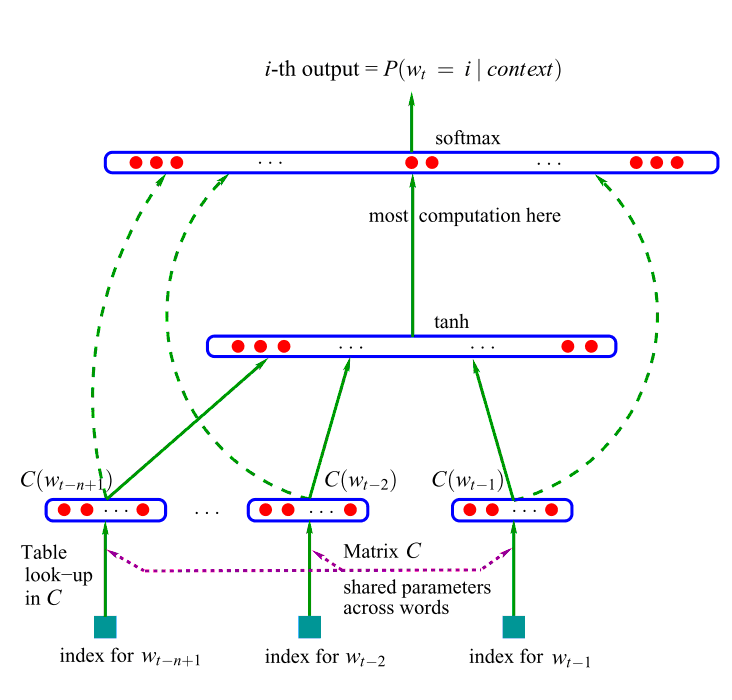
\includegraphics[width=0.7\linewidth]{./figures/nplm.png}
  \caption{前馈神经网络语言模型}\label{fig:nplm}
\end{figure}
图 \ref{fig:nplm} 给出一个典型的 NNLM 语言模型。神经网络语言模型采用普通的三层前馈神经网络结构,其中第一层为输入层。Bengio 提出使用各词的词向量作为输入以解决数据稀疏问题,因此输入层为词$w_{i-(n-1)}; \cdots;w_{i-1} $ 的词向量的顺序拼接:
\begin{equation}\label{equ:we}
  x = [e(w_{i-(n-1)}; \cdots ; e(w_{i-2}); e_{(w_{i-1})}]
\end{equation}
当输入层完成对上文的表示x 之后,模型将其送入剩下两层神经网络,依次得到隐藏层$h$ 和输出层$y$:
\begin{equation}\label{equ:all_nplm}
\begin{split}
h =& tanh(b(1) + Hx) \\
y =& b(2) +Wx + Uh
\end{split}
\end{equation}
其中 $H \in \mathbb{R}^{|h| \times (n-1)|e|}$ 为输入层到隐藏层的权重矩阵,$U \in \mathbb{R}^{|\mathrm{V}|\times (n-1)|h|}$ 为隐藏层到输出层的权重矩阵,$ |\mathrm{V}|$表示词表的大小,$|e|$ 表示词向量的维度,$|g|$ 为隐藏层的维度。$b(1),b(2)$ 均为模型中的偏置项。矩阵$W \in \mathbb{R}^{|\mathcal{V}|\times (n-1)|e|}$ 表示从输入层到输出层的直连边权重矩阵。由于$W$ 的存在,该模型可能会从非线性的神经网络退化成为线性分类器。Bengio 等人在文中指出,如果使用该直连边,可以减少一半的迭代次数;但如果没有直连边,可以生成性能更好的语言模型。因此在后续工作中,很少有使用输入层到输出层直连边的工作,下文也直接忽略这一项。如果不考虑$W$ 矩阵,整个模型计算量最大的操作,就是从隐藏层到输出层的矩阵运算$Uh$,后续的模型均有对这一操作的优化, 这部分内容将在下一节介绍。

\subsection{log 双线性语言模型}
2007 年,Mnih 和Hinton 在神经网络语言模型(NNLM)的基础上提出了log双线性语言模型(Log-Bilinear Language Model,LBL)\cite{DBLP:conf/icml/MnihH07}。LBL 与NNLM 的区别正如它们的名字所示,LBL 的模型结构是一个log 双线性结构;而NNLM的模型结构为神经网络结构。具体来讲,LBL 模型的能量函数为:
\begin{equation}
  E(w_i;w_{i-(n-1):i-1}) = b^{(2)}+ e(wi)^\top b^{(1)}+e(w_i)TH[e(w_{i-(n-1))};\cdots ; e(w_{i-1})
\end{equation}
LBL 模型的能量函数(公式2.14)与NNLM 的能量函数(公式2.11)主要有两个区别。1) LBL 模型中,没有非线性的激活函数tanh,而由于NNLM 是非线性的神经网络结构,激活函数必不可少;2) LBL 模型中,只有一份词向量e,也就是说,无论一个词是作为上下文,还是作为目标词,使用的是同一份词向量。其中第二点(只有一份词向量),只在原版的LBL 模型中存在,后续的改进工作均不包含这一特点。

后来的几年中,Mnih 等人在LBL 模型的基础上做了一系列改进工作。其中最重要的模型有两个:层级log 双线性语言模型(Hierarchical LBL,HLBL)\cite{DBLP:conf/icml/MnihT12} 和基于向量的逆语言模型(inverse vector LBL,ivLBL)\cite{DBLP:conf/nips/MnihK13}。


\subsection{循环神经网络语言模型}
Mikolov等人提出的循环神经网络语言模型(Recurrent Neural Network based Language Model,RNNLM)则直接对$P(w_i | w_1;w_2;\cdots;w_{i-1}) $ 进行建模,而不使用公式 \ref{equ:approx}对其进行简化\cite{mikolov2012statistical,DBLP:conf/interspeech/MikolovKBCK10} 。因此,RNNLM 可以利用所有的上文信息,预测下一个词,其模型结构如图 \ref{fig:rnnlm} 所示。

\begin{figure}
  \centering
  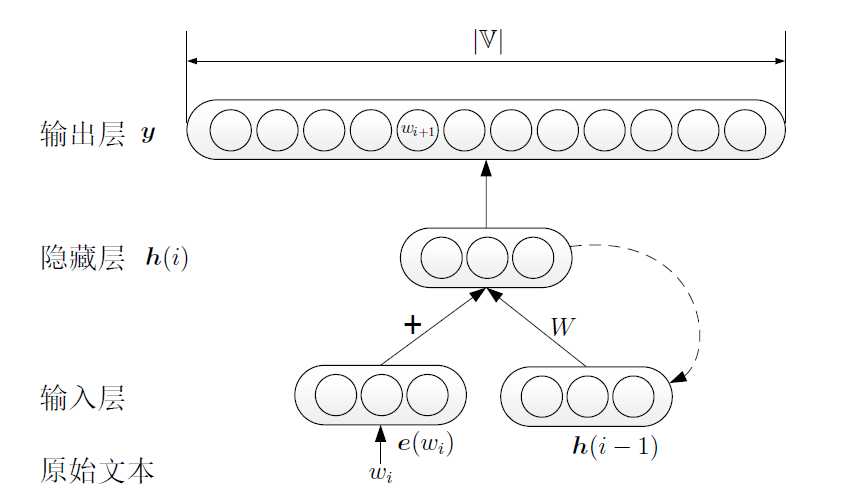
\includegraphics[width=0.85\linewidth]{./figures/rnnlm.png}
  \caption{循环神经网络语言模型(RNNLM)模型结构图}\label{fig:rnnlm}
\end{figure}

RNNLM 的核心在于其隐藏层的算法:
\begin{equation}
\label{equ:rnn}
h(i) =\phi(e(w_i) +Wh(i -1))
\end{equation}
其中,$\phi$非线性激活函数。但与NNLM 不同,RNNLM 并不采用n 元近似,而是使用迭代的方式直接对所有上文进行建模。在公式\ref{equ:rnn} 中,h(i) 表示文本中第$i$ 个词$w_i$ 所对应的隐藏层,该隐藏层由当前词的词向量$e(w_i)$ 以及上一个词对应的隐藏层$h(i -1)$ 结合得到。

隐藏层的初始状态为$h(0)$,随着模型逐个读入语料中的词$w_1;w_2; \cdots $, 隐藏层不断地更新为$h(1);h(2); \cdots$ 。根据公式\ref{equ:rnn},每一个隐藏层包含了当前词的信息以及上一个隐藏层的信息。通过这种迭代推进的方式,每个隐藏层实际上包含了此前所有上文的信息,相比NNLM 只能采用上文n 元短语作为近似,RNNLM 包含了更丰富的上文信息,也有潜力达到更好的效果。RNNLM 的输出层计算方法与NNLM 的输出层一致。


\section{国内外研究现状及发展动态}

\subsection{对上下文信息建模策略}
依照上章节的分析,本章节主要介绍我们实验中所要涉及的模型,主要是各种循环神经网络的变种 \cite{DBLP:conf/icml/JozefowiczZS15}: 普通循环神经网络节点、长短记忆网络(Long shrot-term memory, LSTM) \cite{DBLP:journals/taslp/SundermeyerNS15} 和门限记忆节点(Gated Recurrent Unit, GRU) \cite{DBLP:conf/nips/ChungKDGCB15}。 LSTM的计算公式定于如下 \cite{DBLP:journals/neco/HochreiterS97}:
\begin{itemize}
\item 输入门:输入门:控制当前输入 $x_t$ 和前一步输出 $h_{t−1}$ 进入新的 cell 的信息量:
$$i_t=\sigma(W^i x_t+U^i h_{t-1}+b^i)$$
\item  忘记门:决定是否清楚或者保持单一部分的状态
$$f_t=\sigma(W^f x_t+U^f h_{t-1}+b^f)$$
\item  变换输出和前一状态到最新状态
$$g_t=\phi(W^g x_t+U^g h_{t-1}+b^g)$$
\item  输出门: 计算 cell 的输出
$$o_t=\sigma(W^o x_t+U^o h^{t-1}+b^o)$$
\item  cell 状态更新步骤:计算下一个时间戳的状态使用经过门处理的前一状态和输入:
$$s_t=g_t\odot i_t+s_{t-1}\odot f_t$$
\item  最终 LSTM 的输出:使用一个对当前状态的 tanh 变换进行重变换:
$$h_t=s_t\odot \phi(o_t)$$
\end{itemize}
其中$\odot$ 代表对应元素相乘(Element-wise Matrix Multiplication),$\phi(x), \sigma(x)$ 的定义:

\begin{equation}\label{equ:tanh}
  \phi(x)=\frac{e^x-e^{-x}}{e^x+e^{-x}},\sigma(x)=\frac{1}{1+e^{-x}}
\end{equation}

\begin{figure}
  \centering
  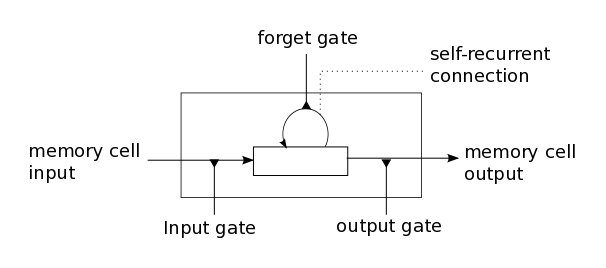
\includegraphics[width=0.9\linewidth]{./figures/lstm_memorycell.png}
  \caption{LSTM 模型}\label{fig:lstm}
\end{figure}


GRU 可以看成是 LSTM 的变种,GRU 把 LSTM中的 forget gate 和 input gate 用 update gate 来替代。 把 cell state 和隐状态 $h_t$ 进行合并,在计算当前时刻新信息的方法和 LSTM 有所不同。 下图是GRU更新 $h_t$ 的过程\cite{DBLP:journals/corr/Pezeshki15}, 具体定义如下:
\begin{itemize}
\item 更新门$z_t$: 定义保存多少以前的信息。

\[z_t = \sigma ( W^z x_t+ U^z h_{t-1}  )\]

\item 重置门$r_t$: 决定保留多少输入信息.

\[r_t = \sigma(W^r x_t  + U^r h_{t-1}  )\]

\item 节点内部更新值$\tilde h_t $: 其次是计算候选隐藏层(candidate hidden layer) $\tilde h_t$,这个候选隐藏层 和LSTM中的$\tilde c_t$是类似,可以看成是当前时刻的新信息,其中$r_t$用来控制需要 保留多少之前的记忆,如果$r_t$为0,那么$\tilde h_t$只包含当前词的信息:
 \[\tilde h_t  = \tanh (W^h x_t  + U^h(h_{t-1} \odot r_t) )\]

\item 隐藏层输出值$h_t$: 最后$z_t$控制需要从前一时刻的隐藏层$h_{t−1}$中遗忘多少信息,需要加入多少当前 时刻的隐藏层信息$\tilde h_t$,最后得到htht,直接得到最后输出的隐藏层信息, 这里与LSTM的区别是GRU中没有 output gate:
\[h_t = (1-z_t)\odot \tilde h_t  + z_t \odot h_{t-1}\]
\end{itemize}
如果reset gate接近0,那么之前的隐藏层信息就会丢弃,允许模型丢弃一些和未来无关 的信息;update gate控制当前时刻的隐藏层输出$h_t$需要保留多少之前的隐藏层信息, 若$z_t$接近1相当于我们之前把之前的隐藏层信息拷贝到当前时刻,可以学习长距离依赖。 一般来说那些具有短距离依赖的单元reset gate比较活跃(如果$r_t$为1,而$z_t$为$0$ 那么相当于变成了一个标准的RNN,能处理短距离依赖),具有长距离依赖的单元update gate比较活跃。

\begin{figure}
  \centering
  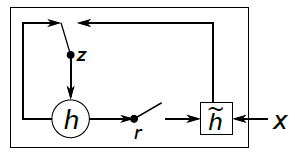
\includegraphics[width=0.6\linewidth]{./figures/gru.png}
  \caption{GRU模型示意图}\label{fig:gru}
\end{figure}


\subsection{对多元分类模型的建模}
大词表问题,主要是对softmax如何建模的问题。在本课题中,我们探讨cHSM和tHSM两种不同的方案所带来的影响和优劣。

传统的多元分类模型(Softmax):
\begin{equation}\label{equ:softmax}
  \hat y_i=\frac{\exp(o_i)}{\sum_j \exp(o_j)}
\end{equation}
其中由于分母是正则项,一旦词表扩大,每次迭代更新都需要计算这一项,是主要的问题所在,所以本课题拟在主要解决该问题所导致的计算费时的问题,在保证计算精度不下降的情况下,提高模型的训练速度。目前主要的策略分为: 基于类别的多元分类模型(class-based hierarchical softmax, cHSM)和基于二叉树的二元分类模型(class-based hierarchical softmax, tHSM).

假设语料中的每一个词样本属于且只属于一个类,在此基础上计算词样本在语料中的分布时,可以先计算类的概率分布,然后在所属类上计算当前词的概率分布,于是可将式(3)转化为

\begin{equation}\label{equ:class}
  p(w_i|h_i) = p(c(t)|h(t))p(w_i|c(t))
\end{equation}
此时,训练一个词样本的计算复杂度正比于:$O =HC$. 式中,C 为语料中所有词的分类数,可根据语料中词的词频进行划分. 当C 取1 或取词典大小V 时,此结构等同于标准的RNN 结构. 由于$C \ll V$,通过图1 结构训练的softmax 降低了计算复杂度.

Mikolov曾提出使用基于二叉树的层级softmax模型来加速的训练方案,加速比能达到理论的最大速度,但是当时提出的背景是基于CPU构建的,如今越来越多的算法随着应用领域的推广,需要在并行度更高的GPU上进行计算,因此基于GPU进行建模的tHSM尚未被研究提及,需要后人研讨。
\subsection{单词聚类的策略}
当我们使用多层分类模型的时候,我们就需要将单词按照模型的架构进行划分。其中对于cHSM模型,我们有以下策略可以使用:1) 基于词频划分类别 2) 基于2-gram 的布朗聚类(brown clustering) 进行划分.3)按照word-embedding 的词向量信息进行聚类。另外,我们还需要注意的是,各个类别可以包含不同的数量的单词,也可以包含数量相同的单词。对于后者,我们考虑的划分模型就是基于交换算法(Exchange Algorithm), 以此来保证获得近似的最优解。 文本聚类方法可以分为静态聚类和动态聚类,静态聚类方法包括Top-down方法和Bottom-up方法,动态聚类(Online clustering)需要判断每个新加入的样本属于已有的类还是一个新类。K-means聚类前提:样本之间相似度能够计算.
Kmeans 算法介绍:
\begin{enumerate}
  \item 随机在图中取$K$个种子点。
  \item 然后对图中的所有点求到这$K$个种子点的距离,假如点$P_i$离种子点$S_i$最近,那么$P_i$属于$S_i$点群。
  \item  接下来,我们要移动种子点到属于他的“点群”的中心;
  \item 然后重复第2)和第3)步,直到种子点没有移动。
\end{enumerate}
K-means缺点:1) 需提前确定聚类数目; 2) 对初始选取的点很敏感; 3) 属于硬聚类(每个样本只能属于一类)



\textbf{熵}:若$X$是一个离散型随机变量,取值空间为$R$,其概率分布为$p(x)=P(X=x),x\in R$。那么,$X$的熵$H(X)$定义为:
\begin{equation}
H(X) = -\sum_{x\in \mathbb{R}}p(x)log_2 p(x)
\end{equation}
其中约定$0log_20 = 0$,通常将$log_2p(x)$写作$logp(x)$。熵又称为自信息,可以视为描述一个随机变量的不确定性的数量。

联合熵和条件熵定义:若$X,Y$是一对离散型随机变量$X,Y ~ p(x,y)$,则$X,Y$的联合熵$H(X,Y)$
\begin{equation}
H(X,Y) = -\sum_{x\in X}\sum_{y\in Y}p(x,y)logp(x,y)
\end{equation}
联合熵实际就是描述一对随机变量平均所需的信息量

给定随机变量$X$的情况下,随机变量$Y$的条件熵如下:
\begin{equation}
H(Y|X) = -\sum_{x\in X}\sum_{y\in Y}p(x,y)log p(y|x)
\end{equation}
条件熵和联合熵的关系:
\begin{equation}
H(X,Y)  = H(Y|X) + H(X)
\end{equation}
推广到一般情况:
\begin{equation}
H(X_1,X_2,...,X_n) = H(X_1)+H(X_2|X_1)+\cdots+H(X_n|X_1,\cdots,X_{n-1})
\end{equation}
互信息
\begin{equation}
H(X,Y) = H(X) + H(Y|X) = H(Y) + H(X|Y)
\end{equation}
可得
\begin{equation}
H(X)-H(X|Y) = H(Y)-H(Y|X)
\end{equation}
这个差称为$X$和$Y$ 的\textbf{互信息},记作$I(X;Y)$,可得$I(X;Y)=H(X)-H(X|Y)$

$I(X;Y)$反映的是在知道了$Y$的值以后$X$的不确定性的减少量。
\begin{figure}
  \centering
  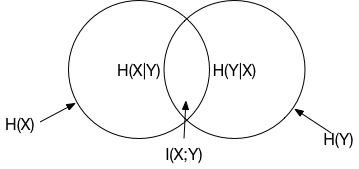
\includegraphics[width=0.5\linewidth]{./figures/mutualInfo.png}
  \caption{互信息示意图}\label{fig:muinfo}
\end{figure}

\begin{equation}
I(X;Y) = \sum_{x,y} p(x,y) log \frac{p(x,y)}{p(x)p(y)}
\end{equation}

\textbf{布朗聚类}:布朗聚类是一种自底而上的层次聚类算法,基于n-gram模型和马尔科夫链模型,是一种硬聚类,每个词都在且只在唯一的一个类中 \cite{derczynski2015tune,DBLP:conf/aaai/DerczynskiC16}。$w$是词,$c$是类,不同于词性标注,此处$c$是未知的。布朗聚类的输入是一个语料库,这个语料库是一个词序列,输出是一个二叉树,树的叶子节点是一个个词,树的中间节点是我们想要的类(中间结点作为根节点的子树上的所有叶子为类中的词)。
\begin{equation}
\begin{split}
Quality(C)=&\frac{1}{n}logP(w_1,\cdots,w_n) =\frac{1}{n}logP(w_1,\cdots,w_n,C(w_1),\cdots,C(w_n))\\
=&\frac{1}{n}log\prod_{i=1}^{n}P(C(w_i)|C(w_{i-1}))P(w_i|C(w_i))\hspace{1.8cm}
\end{split}
\end{equation}
$C(w_0)$是种特殊的\textbf{Start}类,我们要找到这样的分类方式$C$,使得$Quality(C)$尽可能大
\begin{equation}
\begin{split}
Quality(C)=&\frac{1}{n}\sum_{i=1}^{n}P(C(w_i)|C(w_{i-1}))P(w_i|C(w_i))\hspace{3.7cm}\\
=&\sum_{w^{'},w}\frac{n(w,w^{'})}{n}logP(C(w^{'})|C(w)))P(w^{'}|C(w^{'}))\\
=&\sum_{c,c{'}}\frac{n(c,c^{'})}{n}log\frac{n(c,c{'})}{n(c)n(c')}+\sum_{w^{'}} \frac {n(w^{'})}{n}log\frac{n(w')}{n}
\end{split}
\end{equation}
$n(w)$是$w$在文本中出现次数,$n(w,w^{'})$是二元对$w,w^{'}$在文本中的出现次数,$n(c)=\sum_{w\in c}n(w)$,$n(c,c^{'})=\sum_{w\in c}n(w,w^{'})$		
\begin{equation}
  Quality(C) = I(C)-H
\end{equation}

\begin{figure}
  \centering
  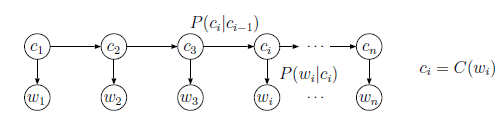
\includegraphics[width=0.9\linewidth]{./figures/brown_clustering.png}
  \caption{布朗聚类示意图}\label{fig:brown}
\end{figure}

\textbf{简单算法:} 以$k$长度文本为例:每个字均为一类,词典大小为$|V|$,找到俩类,合并后使得互信息变得最大,重复合并步骤使得最后都归为一类,整个算法的时间复杂度为$O(|V|^{5})$

\textbf{优化算法:}开始设置一个参数m,比如$m=1000$,我们按照词汇出现的频率对其进行排序然后把频率最高的$m$个词各自分到一个类中,对于第$m+1$到$|V|$个词进行循环:
\begin{enumerate}
  \item 对当前词新建一个类,我们现在又$m+1$个类了
  \item 从这$m+1$个类中贪心选择最好的两个类合并,现在我们剩下$m$个类
  \item 最后我们再做$m-1$词合并。算法时间复杂度$O(|V|*m^2)$
\end{enumerate}


\textbf{哈夫曼树:}在一般的数据结构的书中,树的那章后面,著者一般都会介绍一下哈夫曼(HUFFMAN)树和哈夫曼编码。哈夫曼编码是哈夫曼树的一个应用。哈夫曼编码应用广泛,如JPEG中就应用了哈夫曼编码。

首先介绍什么是哈夫曼树:哈夫曼树又称最优二叉树,是一种带权路径长度最短的二叉树。所谓树的带权路径长度,就是树中所有的叶结点的权值乘上其到根结点的路径长度(若根结点为0层,叶结点到根结点的路径长度为叶结点的层数)。树的带权路径长度记为:
\begin{equation}
WPL=(W1*L1+W2*L2+W3*L3+...+Wn*Ln),
\end{equation}
N个权值$W_i(i=1,2,...n)$构成一棵有N个叶结点的二叉树,相应的叶结点的路径长度为$L_i(i=1,2,...n)$。可以证明哈夫曼树的WPL是最小的。

哈夫曼在上世纪五十年代初就提出这种编码时,根据字符出现的概率来构造平均长度最短的编码。它是一种变长的编码。在编码中,若各码字长度严格按照码字所对应符号出现概率的大小的逆序排列,则编码的平均长度是最小的。(注:码字即为符号经哈夫曼编码后得到的编码,其长度是因符号出现的概率而不同,所以说哈夫曼编码是变长的编码。)

最具有一般规律的构造方法就是哈夫曼算法。一般的数据结构的书中都可以找到其描述:
\begin{enumerate}
  \item 对给定的n个权值$\{W_1,W_2,W_3,\cdots,W_i,\cdots,W_n\}$构成$n$棵二叉树的初始集合$F={T_1,T_2,T_3,\cdots,T_i,\cdots,T_n}$,其中
每棵二叉树$T_i$中只有一个权值为Wi的根结点,它的左右子树均为空。(为方便在计算机上实现算法,一般还要求以Ti的权
值Wi的升序排列。)
\item 在F中选取两棵根结点权值最小的树作为新构造的二叉树的左右子树,新二叉树的根结点的权值为其左右子树的根结点
的权值之和。
\item 从F中删除这两棵树,并把这棵新的二叉树同样以升序排列加入到集合F中。
\item 重复二和三两步,直到集合F中只有一棵二叉树为止。
\end{enumerate}

\textbf{哈夫曼编码}(Huffman Coding)是一种编码方式,以哈夫曼树─即最优二叉树,带权路径长度最小的二叉树,经常应用于数据压缩。 在计算机信息处理中,“哈夫曼编码”是一种一致性编码法(又称"熵编码法"),用于数据的无损耗压缩。这一术语是指使用一张特殊的编码表将源字符(例如某文件中的一个符号)进行编码。这张编码表的特殊之处在于,它是根据每一个源字符出现的估算概率而建立起来的(出现概率高的字符使用较短的编码,反之出现概率低的则使用较长的编码,这便使编码之后的字符串的平均期望长度降低,从而达到无损压缩数据的目的)。这种方法是由David.A.Huffman发展起来的。

例如,在英文中,e的出现概率很高,而z的出现概率则最低。当利用哈夫曼编码对一篇英文进行压缩时,e极有可能用一个位(bit)来表示,而z则可能花去25个位(不是26)。用普通的表示方法时,每个英文字母均占用一个字节(byte),即8个位。二者相比,e使用了一般编码的1/8的长度,z则使用了3倍多。倘若我们能实现对于英文中各个字母出现概率的较准确的估算,就可以大幅度提高无损压缩的比例。


\textbf{霍夫曼算法证明}:构建一棵二叉树,使得最小。
\begin{enumerate}
  \item 首先分析问题的所有解:在叶子数目一定的情况下,二叉树的所有可能是有限的。
\item 假设霍夫曼树是其中最优的,那么它一定比其他树好。我们来进行一次比较。
把叶子节点互换,假设这两个叶子节点的频率为$f1$和$f2$,深度为$d1$和$d2$,互换时,其他叶子节点的cost不变,另为C,那么互换前总cost为$C+f_1d_1+f_2d_2$,互换后为$C+f_1d_2+f_2d_1$,
如果互换后的树变“差”了,那么$f_1d_1+f_2d_2 \le f_1d_2 + f_2d_1$,变换一下即为$f_1(d_1-d_2)\le f_2(d_1-d_2)$
也就是如果$d_1 \le d2$,那么$f_1$必然大于$f_2$,即叶子节点的深度越高,频率必然越低。
那么我们就可以确定最小的俩个叶子节点在最底层。
\item 已经找到了最小的俩个叶子应该怎么放,接下来考虑第三小的叶子。可以继续在底层,也可以放往上一层走。为了解决这个问题,我们进行另一种比较。交换子树,跟(2)中同样的思路,$C+(F_1+F_2)*d_1+F_3*d_2 <= C+F_3*d_1+(F_1+F_2)*d_2$.可以得到,在最优霍夫曼树当中,两个内部节点$n_1$和$n_2$,如果$n_1$比$n_2$更深,那么$n_1$下面的所有叶子的频率之和必然要小于n2下面所有叶子的频率之和。这样的话,我们可以把内部节点的所有叶子的频率之和标在它旁边,那么整棵树的每一个节点就有了一个数值。那么第三小的叶子的情况便可以确定。我们考虑从$(f_1+f_2),f_3,f_4$之选最小的俩个结合为兄弟。
\item 这样就证明霍夫曼算法的递归过程。
\end{enumerate}



\section{总结与展望}
在机器学习领域有一个公认的观点是,模型选用的特征决定了机器学习算法所能达到的上界;而具体模型的选择,则决定了对上界的逼近程度。因此,特征的表示在机器学习中是至关重要的一个步骤。在基于神经网络的语言模型中,尽管不同的模型有着不同的性能,但这些模型均基于分布假说,语义由其上下文决定。这些模型所能表达出的语义,受到语料中各词上下文分布的约束。语言模型的构建是自然语言处理的基础工作,具有重要的理论意义和广阔的应用前景。本文对基于神经网络的语言模型建模技术中,最重要的两个问题,大词表问题和上下文信息的的表示问题,进行深入分析,比较现有方法的优劣。

在基于神经网络的语言模型建模中,本文对现有的语言模型进行了系统的理论对比及实验分析。理论方面,本文阐述了各种现有模型的联系,从上下文的表示、上下文与目标词之间的关系两方面对模型进行了分类整理,并对其中一些重要的模型进行详细描述。在基于神经网络的文档表示技术中,本文分析了现有的文档表示技术:基于循环网络的语言模型和基于前馈神经网络的语言模型。进一步,我们还分析讨论了各种循环神经网络的变种, 例如长短记忆网络和门限循环节点,并绘制模型结构图和具体数学公式。

并针对现有的大词表问题,提出了基于二叉树的多层概率分布函数来提高其效率。该方法克服了传统softmax的计算复杂度过高的问题,但是最初提出来是需要手工构造单词的类别关系。所以利用大数据文本信息,通过聚类算法能否有效提高模型的精确度是值得商榷的实验课题。因此,我们顺便讨论了目前已有的聚类策略,包括:按频率聚类,按照2-gram聚类的布朗聚类算法等等。


最近一两年,已经有人尝试跳出分布假说的框架,使用更广泛的信息,对语义进行建模。Weston 等人设计了一个模型,从知识库中获取语义表示,并用于提升关系抽取任务的性能\cite{DBLP:conf/emnlp/WestonBYU13}。Wang 等人指出,利用知识库中的知识,可以进行词义消歧,进一步提升词向量的性能 \cite{DBLP:conf/emnlp/2014}。未来的工作需要考虑,如何利用海量的多源异构的数据学习到的语言模型,从中挖掘出有用的信息,更好地对数据和知识进行表示。
\newpage
\addcontentsline{toc}{section}{参考文献}
\bibliography{bibs}

\end{document}
